\documentclass[14pt]{article}
\usepackage[utf8]{inputenc}
\usepackage{polski}
\usepackage{extsizes}
\usepackage{amsmath}
\usepackage{amssymb}
\usepackage{graphicx}
\usepackage{enumerate}
\usepackage{mathtools}
\usepackage{setspace}
\usepackage[hmargin=0.6cm, vmargin=2cm, hcentering]{geometry}
\usepackage[export]{adjustbox}
\setlength{\arrayrulewidth}{1mm}
\setlength{\tabcolsep}{18pt}
\renewcommand{\arraystretch}{1.5}
\usepackage[ddmmyyyy]{datetime}
\renewcommand{\dateseparator}{.}
\usepackage{hyperref}
\hypersetup{
    colorlinks=true,
    linkcolor=blue,
    filecolor=magenta,      
    urlcolor=cyan,
}

\begin{document}
\noindent
\rlap{Yevhenii Vinichenko, Krzysztof Wolny} \hfill \hfill \llap{\today}

\begin{center}
\Large {\bf Raport} \\
\large \bf WUM-P2 2021
\end{center}

\section*{Definicja problemu}
Zadaniem tego projektu była klasteryzacja zbioru danych o ludzkiej aktywności fizycznej. Odnośnik do zbioru danych podany jest w sekcji Bibliografia.

\section*{Opis danych}
Zbiór danych zawiera około 10000 rekordów, każdy z których odpowiada pewnej aktywności fizycznej różnych ludzi(leżenie, siedzenie, stojanie, chodzenie, chodzenie po schodach w górę i w dół). Rekordy miały już przypisane etykiety aktywności, z których w czasie klasteryzacji oczywiście nie korzystaliśmy. Każdy rekord miał 561 cech, które były różnego rodzaju statystykami(np. max, min, avg, std itd.) pomiarów, pobranych podczas zbierania danych surowych.

\section*{Preprocessing}
Wykorzystaliśmy już poddane wstępnemu preprocessingowi dane, opis którego znajduje się na stronie, link do której jest w sekcji Bibliografia. Dodatkowo, w celu zmniejszenia wymiarowości, odrzuciliśmy mające zbyt mocno skorelowaną(wartość bezwzględna współczynnika korelacji Pearsona ponad 0.97) parę kolumny(zostało ich tym samym 333), po czym zastosowaliśmy na tym PCA i wybraliśmy 60 piewrszych komponentów(tłumaczyły 91\% wariancji).

\section*{Modelowanie}
Klasteryzację początkowo przeprowadzaliśmy zarówno na danych pierwotnych, jak i przetworzonych przez PCA. Ten drugi wariant reprezentacji danych dawał jednak lepsze wyniki, dlatego ostatecznie skupiliśmy się tylko na nim. Dla wizualizacji klastrów w 2D użyliśmy TSNE. Zastosowaliśmy 4 metody klasteryzujące: KMeans, DBSCAN, GMM oraz aglomeracyjną. Z racji tego, że kmeans dawały najgorsze wyniki, w tym raporcie umieszczamy rezultaty 3 ostatnich metod.
\subsection*{DBSCAN}
Głównym wyzwaniem przy wykorzystaniu tej metody był dobór właściwych wartości \textit{eps} i \textit{min\_samples}. W celu znalezienia \textit{eps} posłużyliśmy się artykułem, link do którego jest w Bibliografii. Artykuł ten polecał policzyć dla każdej obserwacji odległość do jej najbliższego sąsiada, po czym posortować i zestawić te odległości na wykresie. Za dobrą wartość na \textit{eps} uważa się wtedy wartość z osi rzędnych, od której wykres zaczyna drastycznie rosnąć. Podczas liczenia odległości próbowaliśmy metryki euklidesową i Manhattan, ale obie dawały podobne wyniki przy klastrowaniu, więc ostatecznie zostaliśmy przy euklidesowej. Jako \textit{min\_samples} wybraliśmy wartość, która dała najbardziej sensowny wynik z wybranym \textit{eps}(czyli 10).

\begin{figure}[htp]
    \centering
    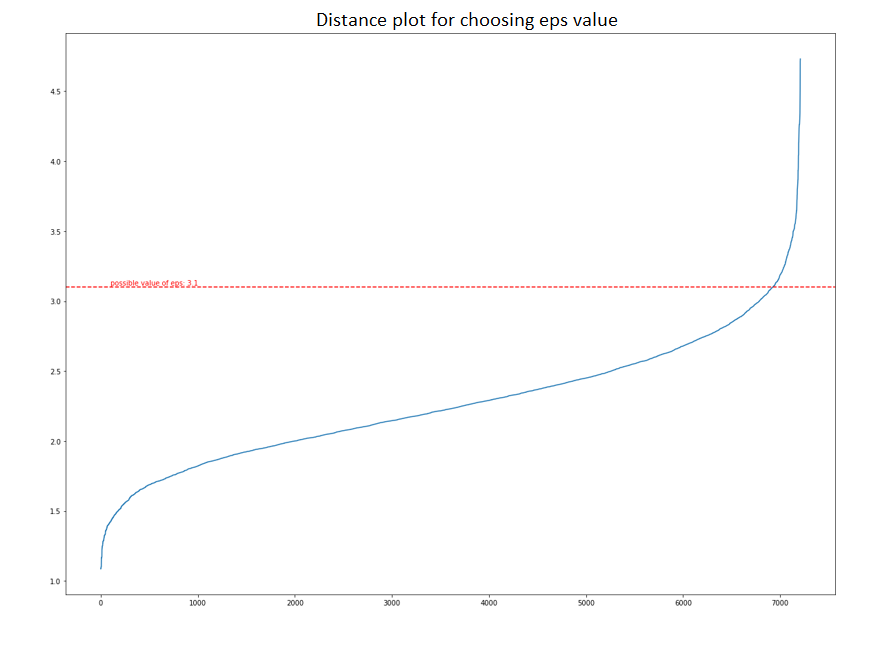
\includegraphics[width=10cm,center]{dbscan1.png}
    \caption{Wykres odległości dla wyboru \textit{eps}}
\end{figure}

\begin{figure}[!htp]
    \centering
    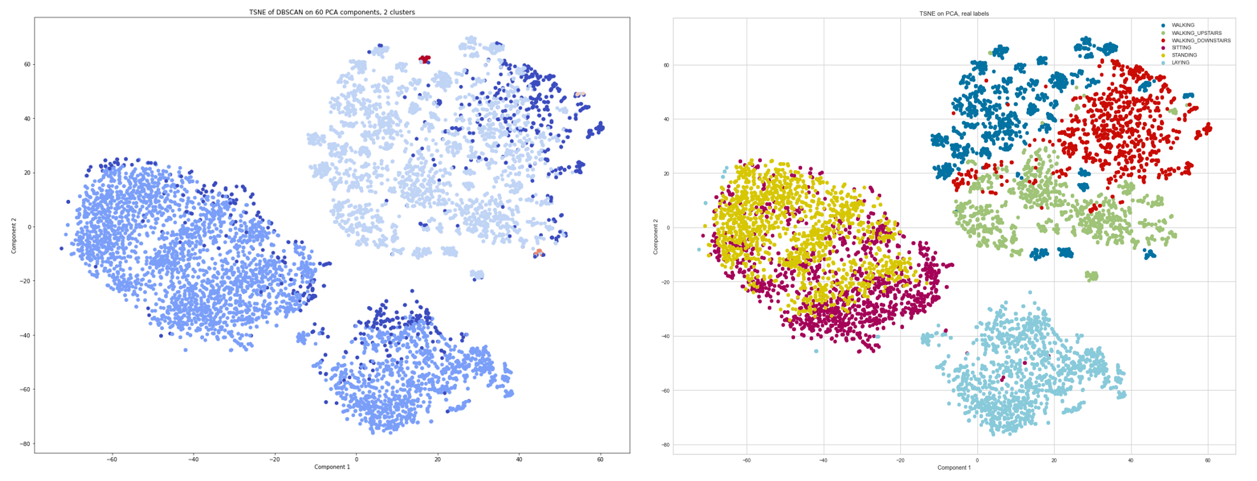
\includegraphics[width=15cm,center]{compare1.png}
    \caption{Porównanie DBSCAN i etykiet oryginalnych}
\end{figure}
\newpage
\noindent
Niestety, wszystko co dało się osiągnąć z DBSCANem, to rozdzielenie aktywności na statyczne i dynamiczne(co w sumie też nie jest złym wynikiem). Powodem tego może być to, że grupy obserwacji wewnątrz każdego z tych ogólnych klastrów nie były dostatecznie gęste, przez co trudno było temu algorytmowi je wykryć. 
\subsection*{Metoda aglomeracyjna}
Tutaj zakładając, że metryki inertia i silhouette są nie najlepszym wyborem dla tego zbioru danych(na etapie testowania KMeans dawały one słabe wyniki dla każdej liczby klastrów, co mogło zachodzić przez to, że szukane klastry nie były wystarczająco kulaste), ograniczyliśmy się do sprawdzenia dendrogramu. Okazało się, że najlepszy link method to metoda Warda(odległości liczyliśmy za pomocą metryki euklidesa)

\begin{figure}[!htp]
    \centering
    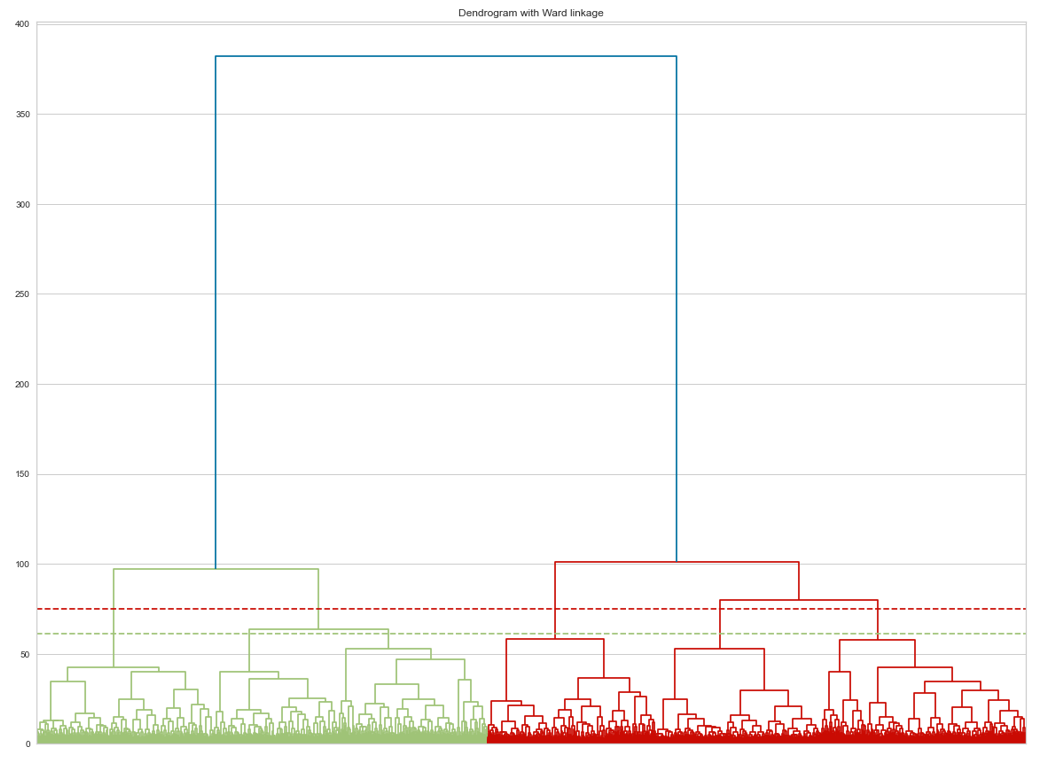
\includegraphics[width=15cm,center]{dendrogram.png}
    \caption{Dendrogram}
\end{figure}
\noindent
Na dendrogramie widać 2 sensowne poziomy odcięcia, wybraliśmy ten zielony(dawało to 6 klastrów).
\newpage
\begin{figure}[!htp]
    \centering
    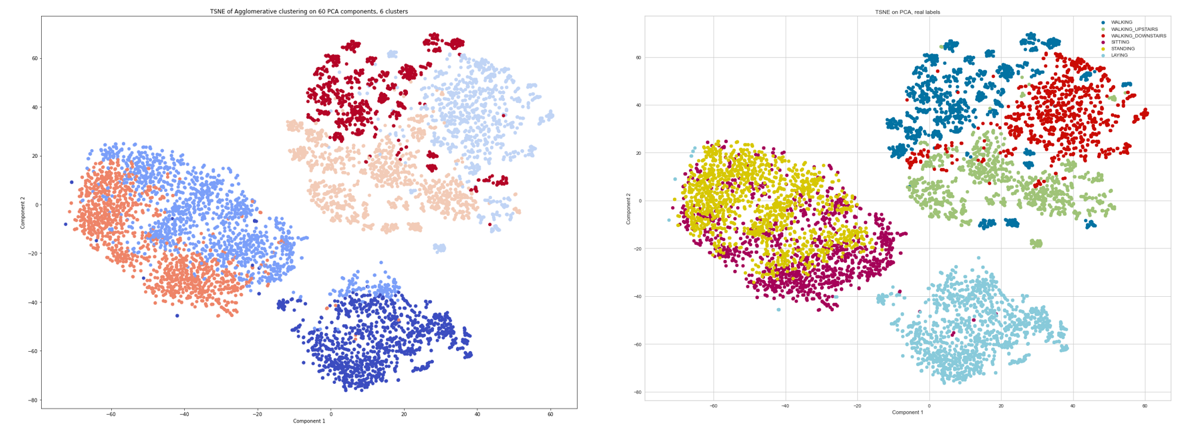
\includegraphics[width=15cm,center]{compare2.png}
    \caption{Porównanie metody aglomeracyjnej i etykiet oryginalnych}
\end{figure}

\subsection*{GMM}
Dla wyboru lepszej liczny klastrów w tej metodzie zdecydowaliśmy jeszcze raz skorzystać z metryki silhouette.

\begin{figure}[!htp]
    \centering
    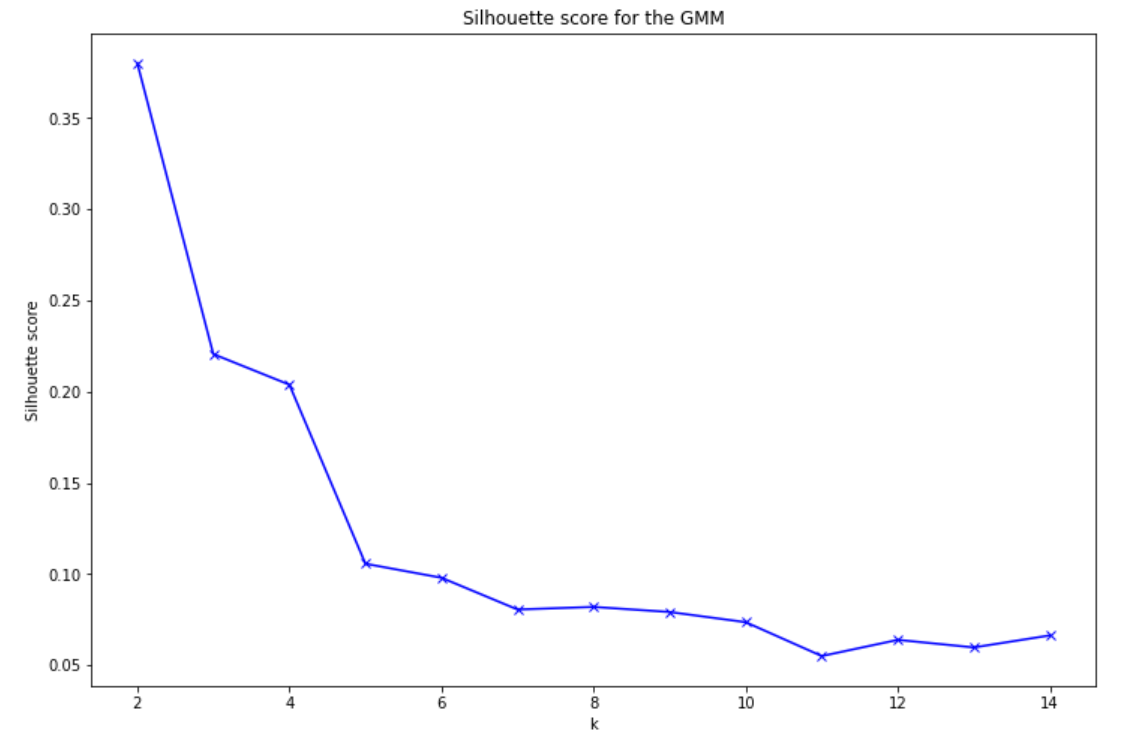
\includegraphics[width=15cm,center]{silhouette.png}
    \caption{Silhouette score dla GMM}
\end{figure}
\noindent
Jak widać, najlepsza liczba klastrów to 2, lecz pamiętając wynik metody aglomeracyjnej, zrobiliśmy też podział na 6 klastrów.
\newpage
\begin{figure}[!htp]
    \centering
    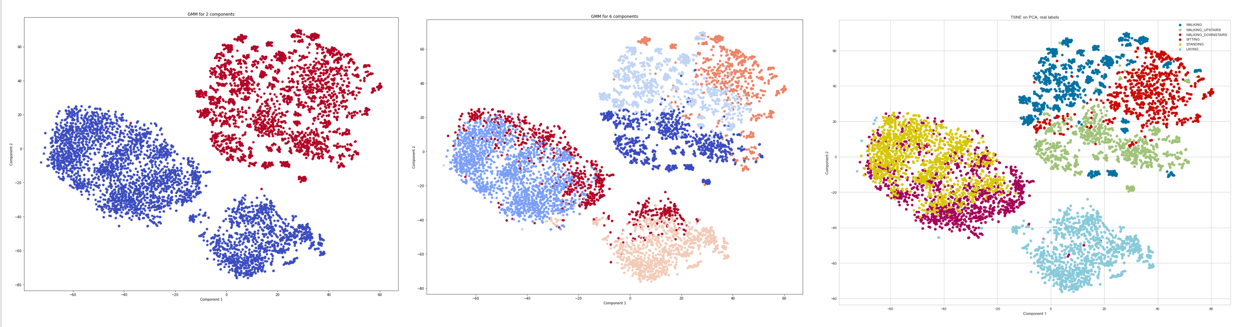
\includegraphics[width=15cm,center]{compare3.png}
    \caption{Porównanie GMM i etykiet oryginalnych}
\end{figure}
\noindent
Podział na 6 klastrów wygląda całkiem porządnie, mimo że silhouette wskazywała, że będzie on fatalny(co jeszcze raz potwierdza, że dla danego zbioru danych jest to nie najlepsza metryka).
\section*{Porównanie z rzeczywistymi etykietami}
Dla najlepiej(przynajmniej wizualnie) prezentującej się metody aglomeracyjnej sprawdziliśmy, jak jej klastry mają się do rzeczywistych etykiet. Najpierw zobaczyliśmy, jak wygląda rozkład etykiet wewnątrz każdego z klastrów, aby utożsamić klastry z etykietami, których w nich jest najwięcej(okazało się, że wtedy każdy klaster faktycznie dostaje inną etykietę). Następnie na zbiorze treningowym(zrobiliśmy podział na samym początku i cały czas działaliśmy na zbiorze treningowym) wytrenowaliśmy KNeighboursClassifier. W jakości zmiennej celu dla każdej obserwacji użyliśmy etykiety jej klastra.

\begin{figure}[!htp]
    \centering
    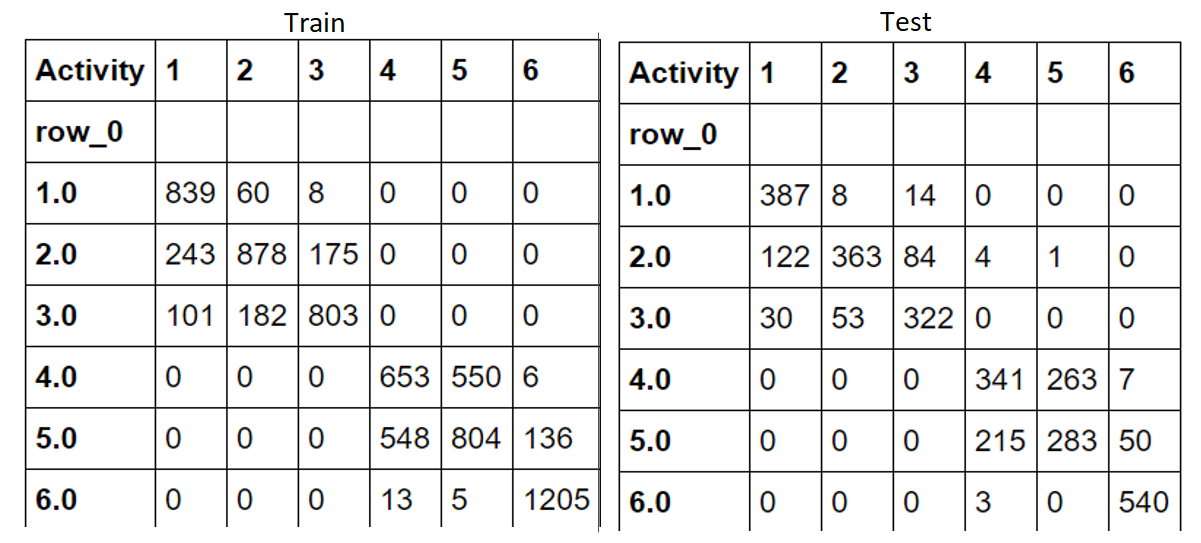
\includegraphics[width=15cm,center]{res.png}
    \caption{Wyniki klasyfikacji na zbiorach treningowym i testowym}
\end{figure}

\section*{Podsumowanie}
Otóż udało nam się wytrenować 2 metody(agglomeracyjną i GMM), które potrafiły stworzyć dostatecznie sensowne podziały danych. Wynikowa liczba klastrów(6) w obu metodach zgadza się z etykietami z oryginalnego zbioru danych. Ponadto klasyfikacja, przeprowadzona za pomocą utworzonego podziału również dała w miarę dobre wyniki. Nie do końca rozwiązaną zostaje kwestia wykorzystania DBSCANa do tego zadania, najprawdopodobniej klastry faktycznie nie są dostatecznie gęste dla tej metody, ale może to być też problem nie najlepiej dobranych hiperparametrów.

\section*{Bibliografia}
\begin{itemize}
    \item Davide Anguita, Alessandro Ghio, Luca Oneto, Xavier Parra and Jorge L. Reyes-Ortiz. A Public Domain Dataset for Human Activity Recognition Using Smartphones. 21th European Symposium on Artificial Neural Networks, Computational Intelligence and Machine Learning, ESANN 2013. Bruges, Belgium 24-26 April 2013, \newline \href{http://archive.ics.uci.edu/ml/datasets/Human+Activity+Recognition+Using+Smartphones}{http://archive.ics.uci.edu/ml/datasets/Human+Activity+Recognition+Using+Smartphones}
    
    \item Dobieranie hiperparametrów dla DBSCAN \newline \href{https://towardsdatascience.com/machine-learning-clustering-dbscan-determine-the-optimal-value-for-epsilon-eps-python-example-3100091cfbc}{https://towardsdatascience.com/machine-learning-clustering-dbscan-determine-the-optimal-value-for-epsilon-eps-python-example-3100091cfbc} 
    \end{itemize}

\end{document}
